% Chapter Template

\chapter{Desarrollo: Iteración I} % Main chapter title

\label{Chapter6} % Change X to a consecutive number; for referencing this chapter elsewhere, use \ref{ChapterX}

\lhead{Capítulo 6. \emph{Iteración I: Configuración y Acción Local}} % Change X to a consecutive number; this is for the header on each page - perhaps a shortened title

%----------------------------------------------------------------------------------------
%	SECTION 1
%----------------------------------------------------------------------------------------
\section{Introducción}

En este capítulo se documentan aspectos relevantes relacionados con la codificación de se realizó en la primera iteración de desarrollo del software.\\
Se plantea la implementación reactiva y genérica de los Casos de Uso. Se expondrá sobre los Schedulers características y empleo.
Se explicaran los Casos de Uso más interesantes de los contemplados para esta iteración.
Se comentará sobre el repositorio de los objetos Módulo, el canal de persistencia local y el de comunicación LAN.

\section{Casos de Uso Reactivo}
Cada caso de uso escrito para la aplicación extenderá la clase abstracta SimpleUseCase o CompletableUseCase que a su vez extiende la definición genérica de un caso de uso reactivo RxUseCase, cuyo código depende fundamentalmente de la librería RxJava.
En la figura ~\ref{fig:class_usecases} se puede ver la relación entre las clases y la definición de los objetos de entrada y salida para cada caso de uso.

\begin{figure}[htbp]
	\centering
	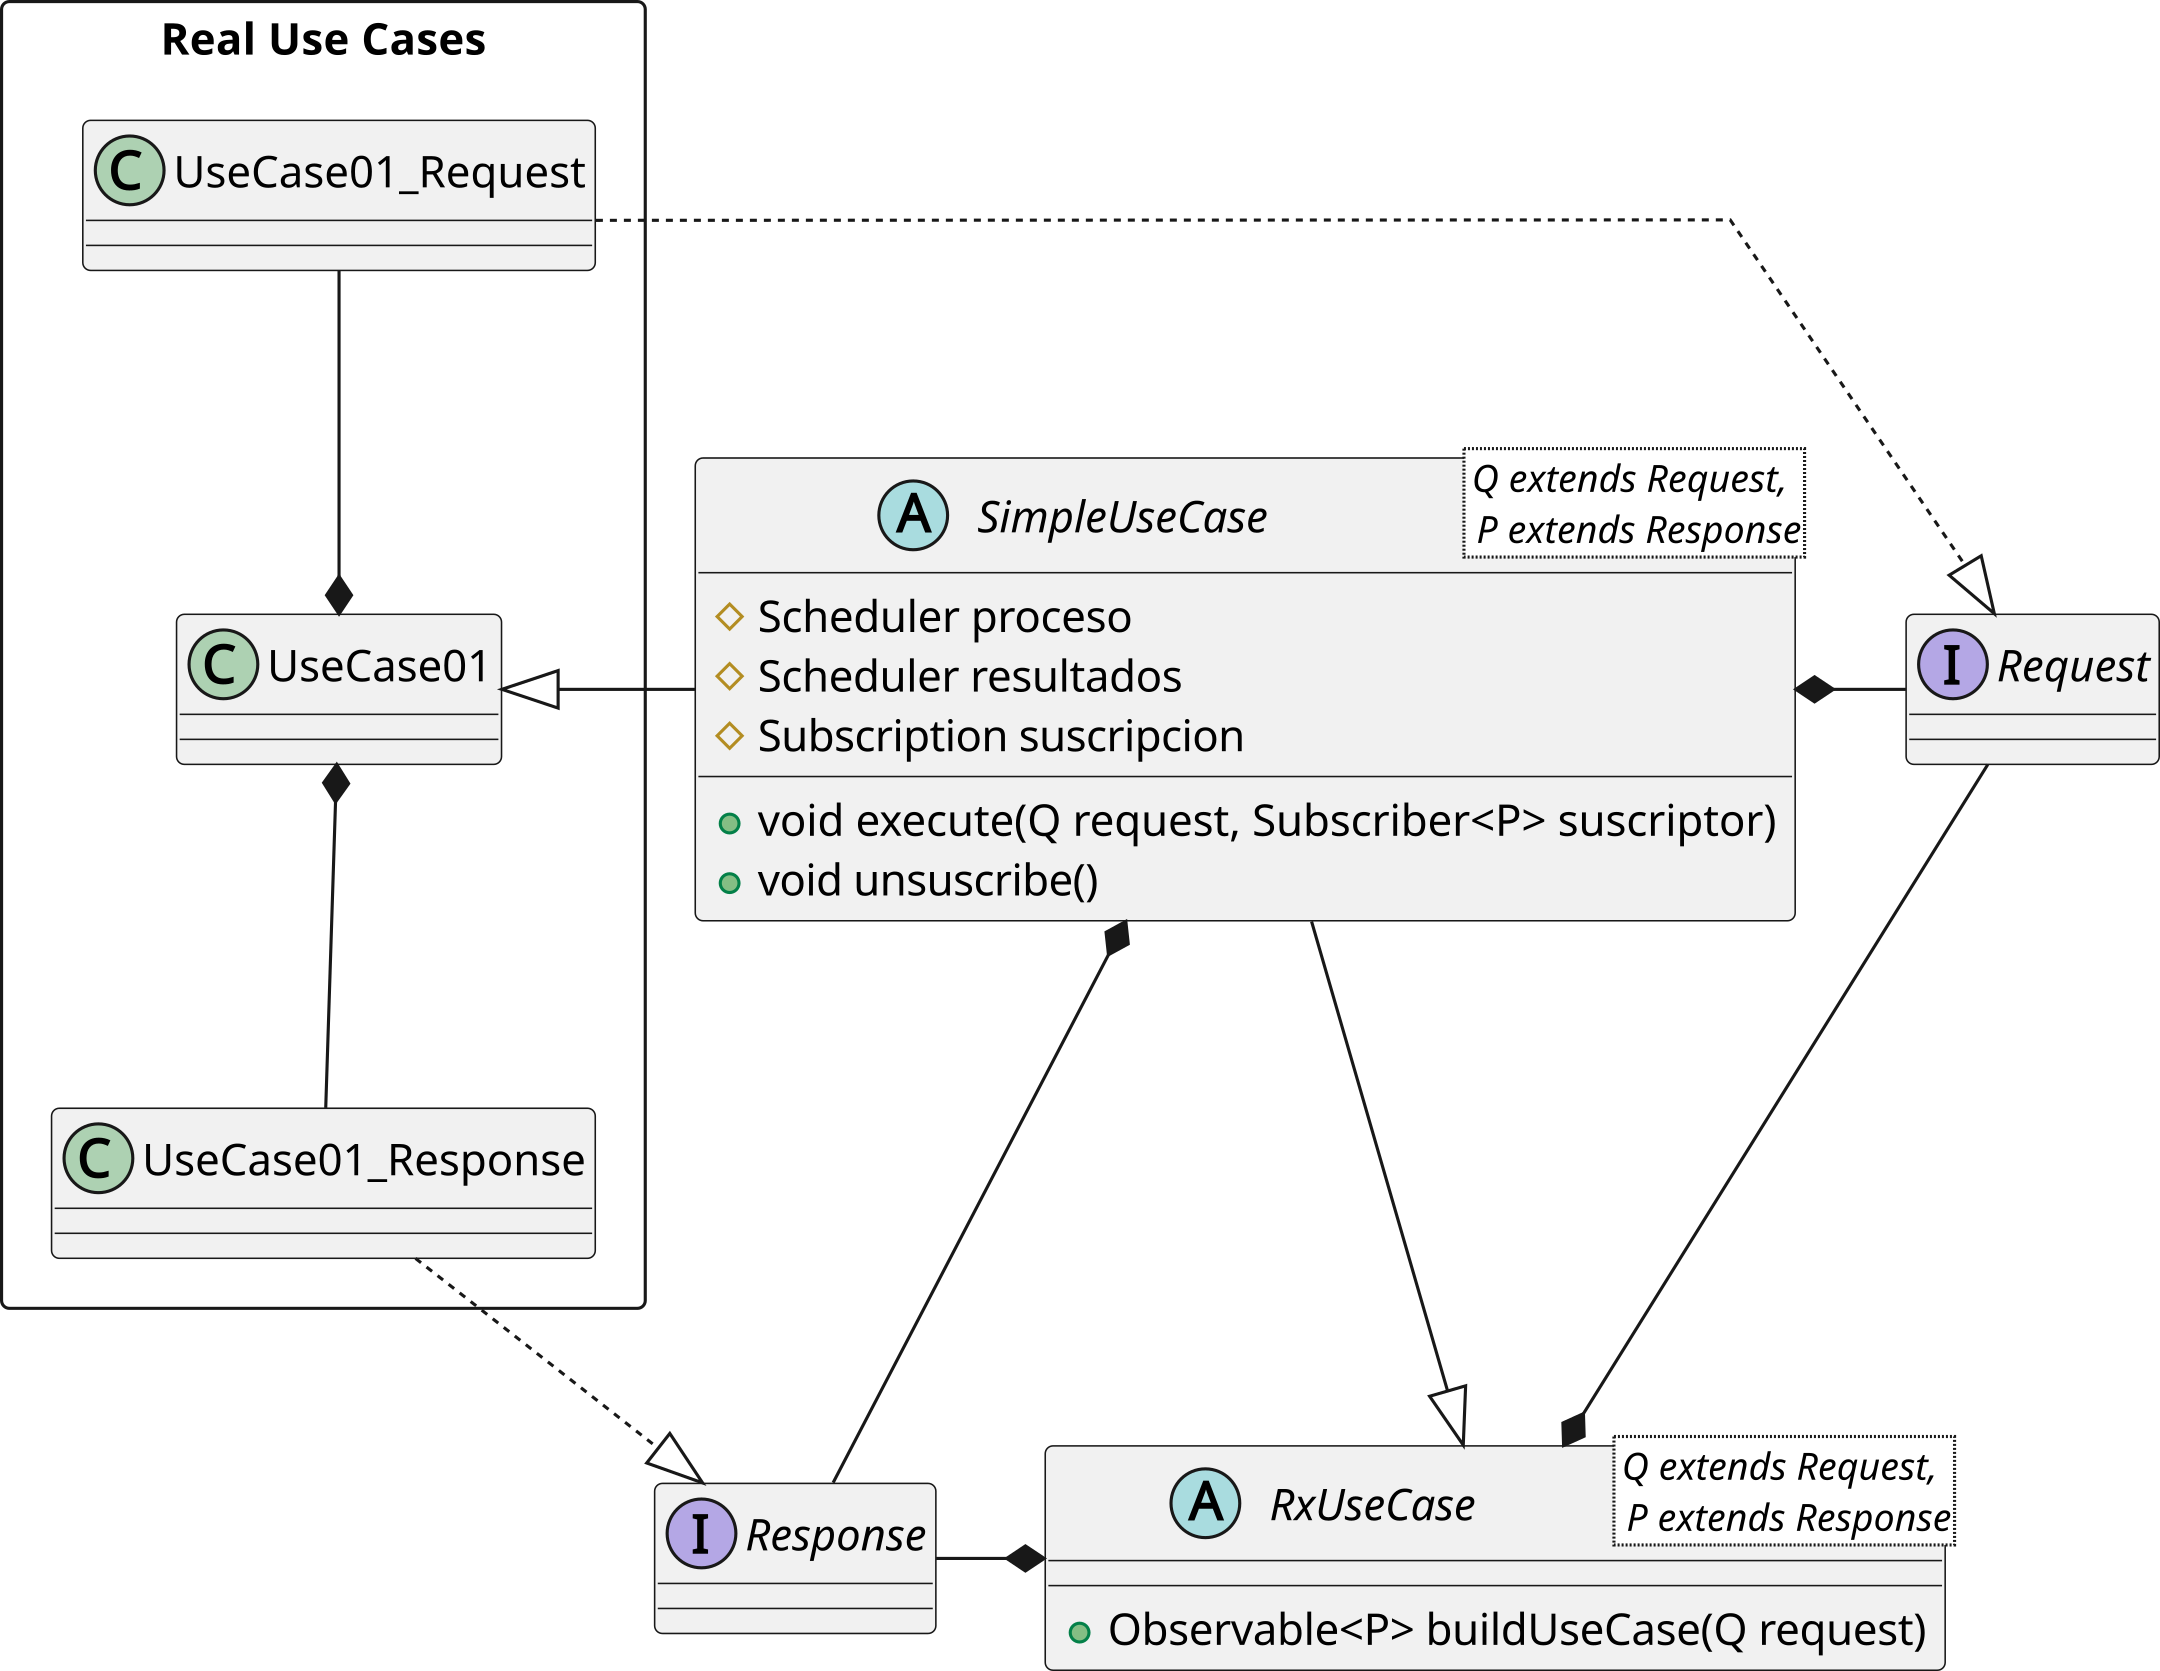
\includegraphics[width=0.8\textwidth]{Figures/iter/CLASS_use_cases.png}
	\rule{35em}{1pt}
	\caption[Class Diagram]{Diagrama de clases de la implementación de un caso de uso.}
	\label{fig:class_usecases}
\end{figure}

\subsection{Schedulers}
En el contexto de la programación reactiva, en particular RxJava, un scheduler (planificador) es un objeto que abstrae el concepto de hilos de ejecución, controla cuándo y en qué hilo se ejecutarán las operaciones de un flujo reactivo. Es decir proveen las instancias de hilos a las que se les asignará las tareas de los operadores en una cadena reactiva. Existen diversos Schedulers implementados por la librería, a saber:

\texttt{Schedulers.io()}\\
Optimizado para operaciones de entrada/salida (I/O) como llamadas de red, lectura/escritura de archivos, acceso a bases de datos, etc.
Usa un grupo de hilos que se expanden según sea necesario para acomodar la carga de trabajo I/O, y reutiliza los hilos cuando están disponibles.

\texttt{Schedulers.computation()}\\
Adecuado para operaciones computacionales que son intensivas en CPU, como cálculos matemáticos complejos.
Usa un número fijo de hilos basado en el número de núcleos del procesador, ya que tener más hilos que núcleos no mejorará el rendimiento para tareas de CPU intensivas.

\texttt{Schedulers.newThread()}\\
Crea un nuevo hilo para cada unidad de trabajo.
No reutiliza hilos, lo que puede llevar a un consumo elevado de recursos si se usa de manera indiscriminada.

\texttt{Schedulers.single()}\\
Ejecuta todas las tareas en un solo hilo.
Útil para operaciones secuenciales donde se necesita garantizar que las tareas se ejecuten en orden sin concurrencia.

\texttt{AndroidSchedulers.mainThread()} (específico de RxAndroid)\\
Usado para ejecutar tareas en el hilo principal (UI thread) en aplicaciones Android.
Asegura que las tareas que interactúan con la UI se ejecuten en el hilo correcto.


Entendido el propósito de emplear schedulers se hace más fácil comprender la implementación del método \texttt{execute()} para la clase \texttt{SimpleUseCase}.
Cada operación de la cadena reactiva generada con \texttt{buildUseCase()} será procesada en un hilo provisto por el planificador para tareas de entrada/salida.
Así mismo las emisiones del resultado final serán capturadas por el hilo principal de la aplicación con el propósito de permitir posibles iteraciones con 
la interfaz de usuario. 

\begin{lstlisting}[caption={Método execute SimpleUseCase}, label={code:exec_usecase}, language=java, basicstyle=\ttfamily \footnotesize, numbers=left, stepnumber=1, showstringspaces=false, float]
public void execute(Q requestValues, Subscriber<P> subscriber) {
	unsubscribe();
	mSubscription = buildUseCase(requestValues)
		.subscribeOn(this.mSubscribeOn)
		.observeOn(this.mObserveOn)
		.subscribe(subscriber);
}
\end{lstlisting}

Este modo de operación multithread se especifica en las lineas 5 y 6 del código implementado para el método \texttt{excecute()} ~\ref{code:exec_usecase}
al llamar al método \texttt{subscribeOn()} se establece que todas las operaciones de la cadena reactiva se realizaran en un hilo provisto por el scheduler de E/S mientras que al llamar al método \texttt{observeOn()} como ultima operación de la cadena se fija el hilo principal de la aplicación como capturador de las emisiones del flujo de datos.

\section{Casos de Uso Implementados}
Para la presente iteración se implementaron los siguientes casos de uso.
\begin{enumerate}
	\item Buscar Módulos disponibles
	\item Solicitar Acceso
	\item Accionar Módulo
	\item Obtener datos de módulo
	\item Resetear a valores de fábrica
	\item Ingresar Credenciales WiFi
	\item Cambiar Alias	
\end{enumerate}

A continuación se documentaran aquellos que presentan los escenarios más interesantes.

\subsection{Solicitar acceso a Módulo}
Un nuevo usuario instala la aplicación cliente en su teléfono android.
Después de registrar su número telefónico, busca los módulos disponibles en la red local.
Encuentra uno y procede a solicitar acceso para que algún administrador lo autorice.
Esta operación puede utilizar hasta dos RPCs en su ejecución y puede fallar en 5 escenarios:
\begin{itemize}
	\item Error de comunicación con el módulo
	\item El módulo tuvo un error al intentar registrar al usuario
	\item Se alcanzó el máximo de usuarios admitidos por el módulo
	\item Improbable caso donde un administrador autoriza y elimina de inmediato al solicitante.
\end{itemize}
Para los escenarios 1 y 3 se permite la posibilidad de reintentar la operación una vez.
En el diagrama de la figura ~\ref{fig:act_request} se puede observar el flujo del algoritmo implementado para este caso de uso.

\begin{figure}[htbp]
	\centering
	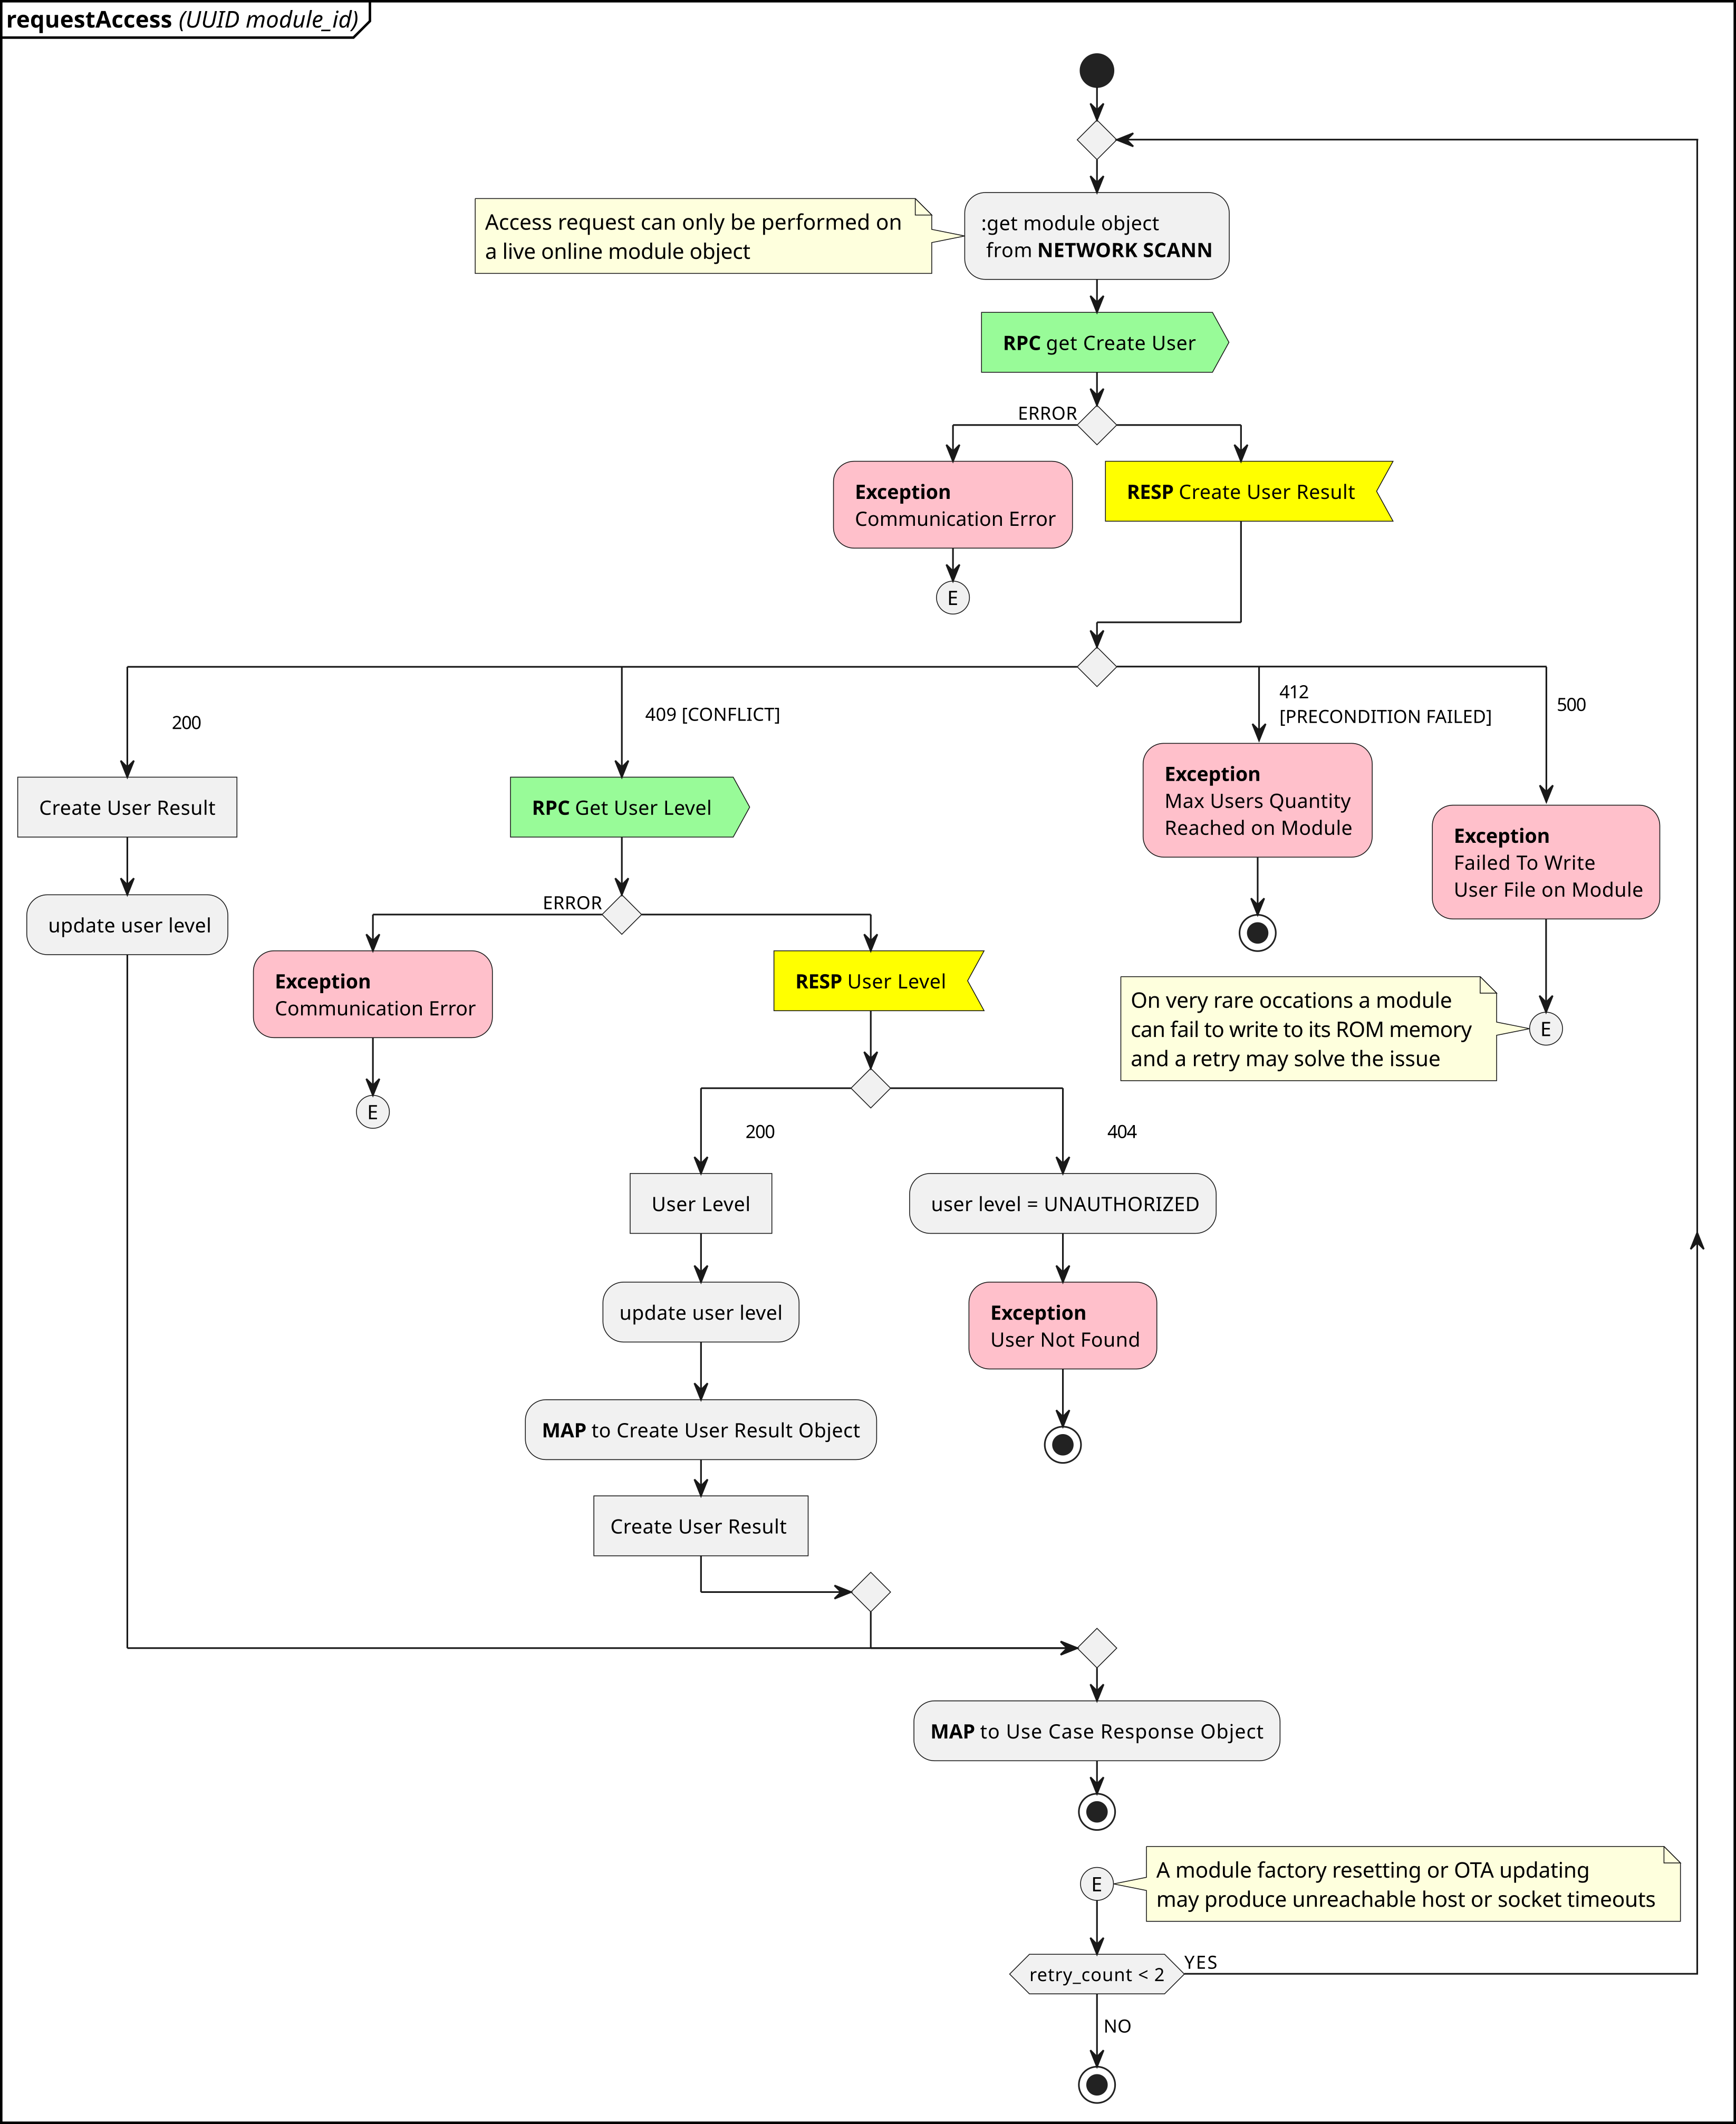
\includegraphics[width=\textwidth]{Figures/iter/ACT_request_ink.png}
	\rule{35em}{1pt}
	\caption[Class Diagram]{Diagrama de actividades de la implementación del caso de uso: Solicitar Acceso.}
	\label{fig:act_request}
\end{figure}

\subsection{Accionar Módulo}

\subsection{Obtener datos del Módulo}


\section{Conclusión}